\documentclass{standalone}
\usepackage{tikz}
\usetikzlibrary{patterns, positioning}


\begin{document}
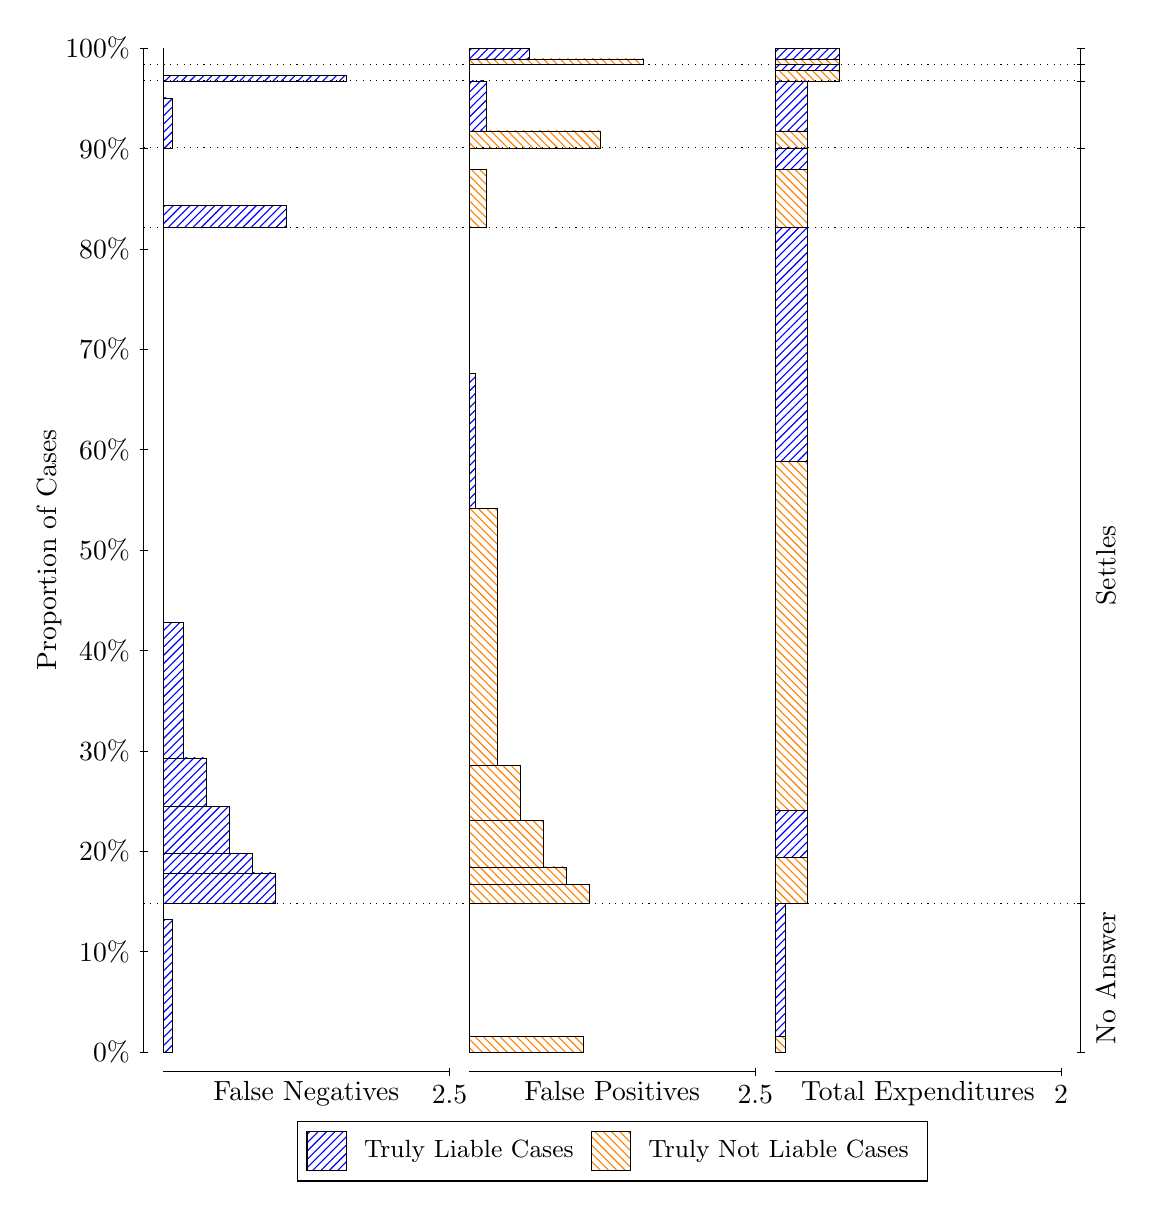
\begin{tikzpicture}
\draw[black, very thin] (1.5,1.75) -- (1.5,14.5);
\node[rotate=90, text=black, anchor=center] at (0.3, 8.125) {Proportion of Cases};
\draw[black, very thin] (1.45,1.75) -- (1.55,1.75);
\node[text=black, anchor=east] at (1.45, 1.75) {0\%};
\draw[black, very thin] (1.45,3.025) -- (1.55,3.025);
\node[text=black, anchor=east] at (1.45, 3.025) {10\%};
\draw[black, very thin] (1.45,4.3) -- (1.55,4.3);
\node[text=black, anchor=east] at (1.45, 4.3) {20\%};
\draw[black, very thin] (1.45,5.575) -- (1.55,5.575);
\node[text=black, anchor=east] at (1.45, 5.575) {30\%};
\draw[black, very thin] (1.45,6.85) -- (1.55,6.85);
\node[text=black, anchor=east] at (1.45, 6.85) {40\%};
\draw[black, very thin] (1.45,8.125) -- (1.55,8.125);
\node[text=black, anchor=east] at (1.45, 8.125) {50\%};
\draw[black, very thin] (1.45,9.4) -- (1.55,9.4);
\node[text=black, anchor=east] at (1.45, 9.4) {60\%};
\draw[black, very thin] (1.45,10.675) -- (1.55,10.675);
\node[text=black, anchor=east] at (1.45, 10.675) {70\%};
\draw[black, very thin] (1.45,11.95) -- (1.55,11.95);
\node[text=black, anchor=east] at (1.45, 11.95) {80\%};
\draw[black, very thin] (1.45,13.225) -- (1.55,13.225);
\node[text=black, anchor=east] at (1.45, 13.225) {90\%};
\draw[black, very thin] (1.45,14.5) -- (1.55,14.5);
\node[text=black, anchor=east] at (1.45, 14.5) {100\%};

\draw[black, very thin] (13.4,1.75) -- (13.4,14.5);
\draw[black, very thin] (13.35,1.75) -- (13.45,1.75);
\node[anchor=west] at (13.35, 1.75) {};
\draw[black, very thin] (13.35,3.6342) -- (13.45,3.6342);
\node[anchor=west] at (13.35, 3.6342) {};
\draw[black, very thin] (13.35,12.222) -- (13.45,12.222);
\node[anchor=west] at (13.35, 12.222) {};
\draw[black, very thin] (13.35,13.233) -- (13.45,13.233);
\node[anchor=west] at (13.35, 13.233) {};
\draw[black, very thin] (13.35,14.083) -- (13.45,14.083);
\node[anchor=west] at (13.35, 14.083) {};
\draw[black, very thin] (13.35,14.289) -- (13.45,14.289);
\node[anchor=west] at (13.35, 14.289) {};
\draw[black, very thin] (13.35,14.5) -- (13.45,14.5);
\node[anchor=west] at (13.35, 14.5) {};

\draw[black, very thin, pattern color=blue, pattern=north east lines] (1.75,1.75) rectangle (1.859,3.436);
\draw[black, very thin, pattern color=orange, pattern=north west lines] (1.75,3.436) rectangle (1.75,3.6342);
\draw[black, very thin, pattern color=blue, pattern=north east lines] (1.75,3.6342) rectangle (3.167,4.023);
\draw[black, very thin, pattern color=blue, pattern=north east lines] (1.75,4.023) rectangle (2.8763,4.2694);
\draw[black, very thin, pattern color=blue, pattern=north east lines] (1.75,4.2694) rectangle (2.5857,4.8646);
\draw[black, very thin, pattern color=blue, pattern=north east lines] (1.75,4.8646) rectangle (2.295,5.484);
\draw[black, very thin, pattern color=blue, pattern=north east lines] (1.75,5.484) rectangle (2.0043,7.203);
\draw[black, very thin, pattern color=orange, pattern=north west lines] (1.75,7.203) rectangle (1.75,12.222);
\draw[black, very thin, pattern color=blue, pattern=north east lines] (1.75,12.222) rectangle (3.3123,12.497);
\draw[black, very thin, pattern color=orange, pattern=north west lines] (1.75,12.497) rectangle (1.75,13.233);
\draw[black, very thin, pattern color=blue, pattern=north east lines] (1.75,13.233) rectangle (1.859,13.868);
\draw[black, very thin, pattern color=orange, pattern=north west lines] (1.75,13.868) rectangle (1.75,14.083);
\draw[black, very thin, pattern color=blue, pattern=north east lines] (1.75,14.083) rectangle (4.0753,14.157);
\draw[black, very thin, pattern color=orange, pattern=north west lines] (1.75,14.157) rectangle (1.75,14.289);
\draw[black, very thin, pattern color=orange, pattern=north west lines] (1.75,14.289) rectangle (1.75,14.362);
\draw[black, very thin, pattern color=blue, pattern=north east lines] (1.75,14.362) rectangle (1.75,14.5);
\draw[black, very thin, pattern color=orange, pattern=north west lines] (5.6333,1.75) rectangle (7.0867,1.9482);
\draw[black, very thin, pattern color=blue, pattern=north east lines] (5.6333,1.9482) rectangle (5.6333,3.6342);
\draw[black, very thin, pattern color=orange, pattern=north west lines] (5.6333,3.6342) rectangle (7.1593,3.8748);
\draw[black, very thin, pattern color=orange, pattern=north west lines] (5.6333,3.8748) rectangle (6.8687,4.1011);
\draw[black, very thin, pattern color=orange, pattern=north west lines] (5.6333,4.1011) rectangle (6.578,4.6867);
\draw[black, very thin, pattern color=orange, pattern=north west lines] (5.6333,4.6867) rectangle (6.2873,5.3896);
\draw[black, very thin, pattern color=orange, pattern=north west lines] (5.6333,5.3896) rectangle (5.9967,8.6534);
\draw[black, very thin, pattern color=blue, pattern=north east lines] (5.6333,8.6534) rectangle (5.706,10.372);
\draw[black, very thin, pattern color=blue, pattern=north east lines] (5.6333,10.372) rectangle (5.6333,12.222);
\draw[black, very thin, pattern color=orange, pattern=north west lines] (5.6333,12.222) rectangle (5.8513,12.959);
\draw[black, very thin, pattern color=blue, pattern=north east lines] (5.6333,12.959) rectangle (5.6333,13.233);
\draw[black, very thin, pattern color=orange, pattern=north west lines] (5.6333,13.233) rectangle (7.3047,13.449);
\draw[black, very thin, pattern color=blue, pattern=north east lines] (5.6333,13.449) rectangle (5.8513,14.083);
\draw[black, very thin, pattern color=orange, pattern=north west lines] (5.6333,14.083) rectangle (5.6333,14.216);
\draw[black, very thin, pattern color=blue, pattern=north east lines] (5.6333,14.216) rectangle (5.6333,14.289);
\draw[black, very thin, pattern color=orange, pattern=north west lines] (5.6333,14.289) rectangle (7.8497,14.362);
\draw[black, very thin, pattern color=blue, pattern=north east lines] (5.6333,14.362) rectangle (6.3963,14.5);
\draw[black, very thin, pattern color=orange, pattern=north west lines] (9.5167,1.75) rectangle (9.6529,1.9482);
\draw[black, very thin, pattern color=blue, pattern=north east lines] (9.5167,1.9482) rectangle (9.6529,3.6342);
\draw[black, very thin, pattern color=orange, pattern=north west lines] (9.5167,3.6342) rectangle (9.9254,4.2198);
\draw[black, very thin, pattern color=blue, pattern=north east lines] (9.5167,4.2198) rectangle (9.9254,4.815);
\draw[black, very thin, pattern color=orange, pattern=north west lines] (9.5167,4.815) rectangle (9.9254,9.2486);
\draw[black, very thin, pattern color=blue, pattern=north east lines] (9.5167,9.2486) rectangle (9.9254,12.222);
\draw[black, very thin, pattern color=orange, pattern=north west lines] (9.5167,12.222) rectangle (9.9254,12.959);
\draw[black, very thin, pattern color=blue, pattern=north east lines] (9.5167,12.959) rectangle (9.9254,13.233);
\draw[black, very thin, pattern color=orange, pattern=north west lines] (9.5167,13.233) rectangle (9.9254,13.449);
\draw[black, very thin, pattern color=blue, pattern=north east lines] (9.5167,13.449) rectangle (9.9254,14.083);
\draw[black, very thin, pattern color=orange, pattern=north west lines] (9.5167,14.083) rectangle (10.334,14.216);
\draw[black, very thin, pattern color=blue, pattern=north east lines] (9.5167,14.216) rectangle (10.334,14.289);
\draw[black, very thin, pattern color=orange, pattern=north west lines] (9.5167,14.289) rectangle (10.334,14.362);
\draw[black, very thin, pattern color=blue, pattern=north east lines] (9.5167,14.362) rectangle (10.334,14.5);
\draw[black, dotted] (1.5,3.6342) -- (13.4,3.6342);
\draw[black, dotted] (1.5,12.222) -- (13.4,12.222);
\draw[black, dotted] (1.5,13.233) -- (13.4,13.233);
\draw[black, dotted] (1.5,14.083) -- (13.4,14.083);
\draw[black, dotted] (1.5,14.289) -- (13.4,14.289);
\draw[black, very thin] (1.75,1.5) -- (5.3833,1.5);
\node[text=black, anchor=north] at (3.5667, 1.5) {False Negatives};
\draw[black, very thin] (5.3833,1.45) -- (5.3833,1.55);
\node[text=black, anchor=north] at (5.3833, 1.45) {2.5};

\draw[black, very thin] (5.6333,1.5) -- (9.2667,1.5);
\node[text=black, anchor=north] at (7.45, 1.5) {False Positives};
\draw[black, very thin] (9.2667,1.45) -- (9.2667,1.55);
\node[text=black, anchor=north] at (9.2667, 1.45) {2.5};

\draw[black, very thin] (9.5167,1.5) -- (13.15,1.5);
\node[text=black, anchor=north] at (11.333, 1.5) {Total Expenditures};
\draw[black, very thin] (13.15,1.45) -- (13.15,1.55);
\node[text=black, anchor=north] at (13.15, 1.45) {2};

\node[text=black, centered, rotate=90] at (13.72, 2.6921) {No Answer};
\node[text=black, centered, rotate=90] at (13.72, 7.9282) {Settles};





\draw (7.449999999999999,1.5) node[draw=none] (baseCoordinate) {};
\begin{scope}[align=center]
        \matrix[scale=0.5, draw=black, below=0.5cm of baseCoordinate, nodes={draw}, column sep=0.1cm]{
            \node[rectangle, draw, minimum width=0.5cm, minimum height=0.5cm, pattern color=blue, pattern=north east lines] {}; &
            \node[draw=none, font=\small, text=black] (B) {Truly Liable Cases}; &
            \node[rectangle, draw, minimum width=0.5cm, minimum height=0.5cm, pattern color=orange, pattern=north west lines] {}; &
            \node[draw=none, font=\small, text=black] (B) {Truly Not Liable Cases}; \\
            };
\end{scope}

\end{tikzpicture}
\end{document}